\documentclass{beamer}
\usetheme{metropolis}           % Use metropolis theme
\usepackage{appendixnumberbeamer}
\usepackage{epigraph}
\usepackage{color}
\usepackage{amsopn}
\usepackage{tabto}
\usepackage{pbox}           % table line break
\usepackage{algorithm}      % algorithm
\usepackage[noend]{algpseudocode} % algorithm
\usepackage{bm}             % bold in math
\usepackage{mathtools}      % dcases*

%%% Bibliography
\usepackage[backend=bibtex, style=authoryear]{biblatex}
\AtBeginBibliography{\tiny}
\bibliography{../bibliography.bib}

\setcounter{tocdepth}{1}      % hide subsections in Table of Contents
\renewcommand{\thealgorithm}{} % disable numbering of algorithms

\setbeamercolor{background canvas}{bg=white}
\setbeamercolor{title}{fg=gray!10}
\setbeamercolor{subtitle}{fg=gray!15}
\setbeamercolor{author}{fg=gray!40}
\setbeamercolor{date}{fg=gray!60}
\setbeamercolor{institute}{fg=gray!20}

\newcommand{\todo}{\alert{TODO}}
\newcommand{\itemBullet}{\scriptsize$\blacksquare$}
\setbeamertemplate{itemize item}{\itemBullet}
\setbeamertemplate{itemize subitem}{\itemBullet}
\setbeamertemplate{itemize subsubitem}{\itemBullet}
\newcommand{\E}{\mathop{\mathbb{E}}}
\DeclareMathOperator*{\argmax}{arg\,max}
\newcommand{\epiParSpace}{\vskip 1.5ex}
\newcommand{\p}{\mathbf{p}}
\newcommand{\colorcite}{\color{gray!35}}

\title{Dynamic Routing Between Capsules}
\subtitle{by S. Sabour, N. Frosst and G. Hinton (NIPS 2017)}
\author{presented by Karel Ha}
\date{27\textsuperscript{th} March 2018}                         % no dates
\institute{Pattern Recognition and Computer Vision Reading Group}

\begin{document}
  {
    \usebackgroundtemplate{
      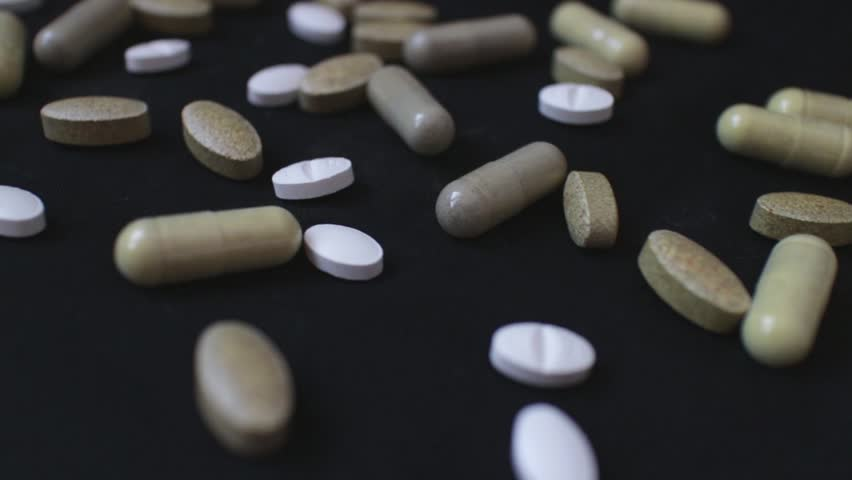
\includegraphics[height=\paperheight]{../img/capsule-pills.jpg}
    }
    \maketitle
  }

  \begin{frame}{Outline}
    \tableofcontents
  \end{frame}

%%%%%%%%%%%%%%%%%%%%%%%%%%%%%%%%%%%%%%%%%%%%%%%%%%%%%%%%%%%%%%%%%%%%%%%%%%%%%%%%

  \section{Motivation}
  {
    \setbeamertemplate{frame footer}{\colorcite\url{https://medium.com/ai³-theory-practice-business/understanding-hintons-capsule-networks-part-i-intuition-b4b559d1159b}}

    \begin{frame}{Geometric Relationships between the Whole and Its Parts}
      \begin{center}
        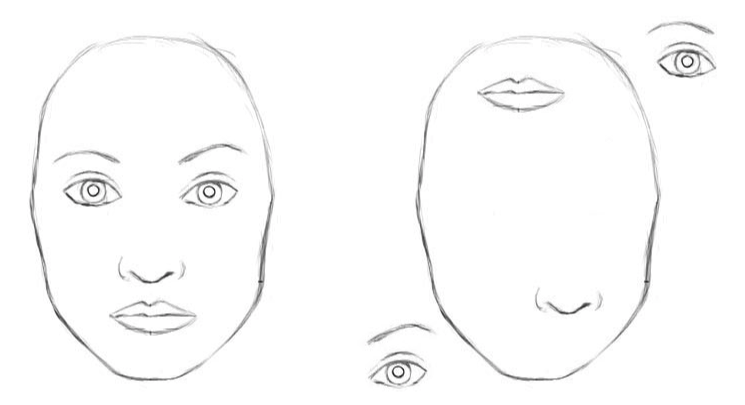
\includegraphics[width=\textwidth]{../img/ambiguous-faces.png}
      \end{center}
      \pause
      To a CNN, both pictures are similar, since they both contain similar elements.
    \end{frame}
  }

  \subsection{Prior Work}

%%%%%%%%%%%%%%%%%%%%%%%%%%%%%%%%%%%%%%%%%%%%%%%%%%%%%%%%%%%%%%%%%%%%%%%%%%%%%%%%

  \section{Capsule}

  \subsection{CapsNets vs ConvNets}
  {
    \setbeamertemplate{frame footer}{\colorcite[\cite{Sabour2017dynamic}]}

    \begin{frame}{Where ConvNets Ends... And CapsNets Begins...}
      \begin{center}
        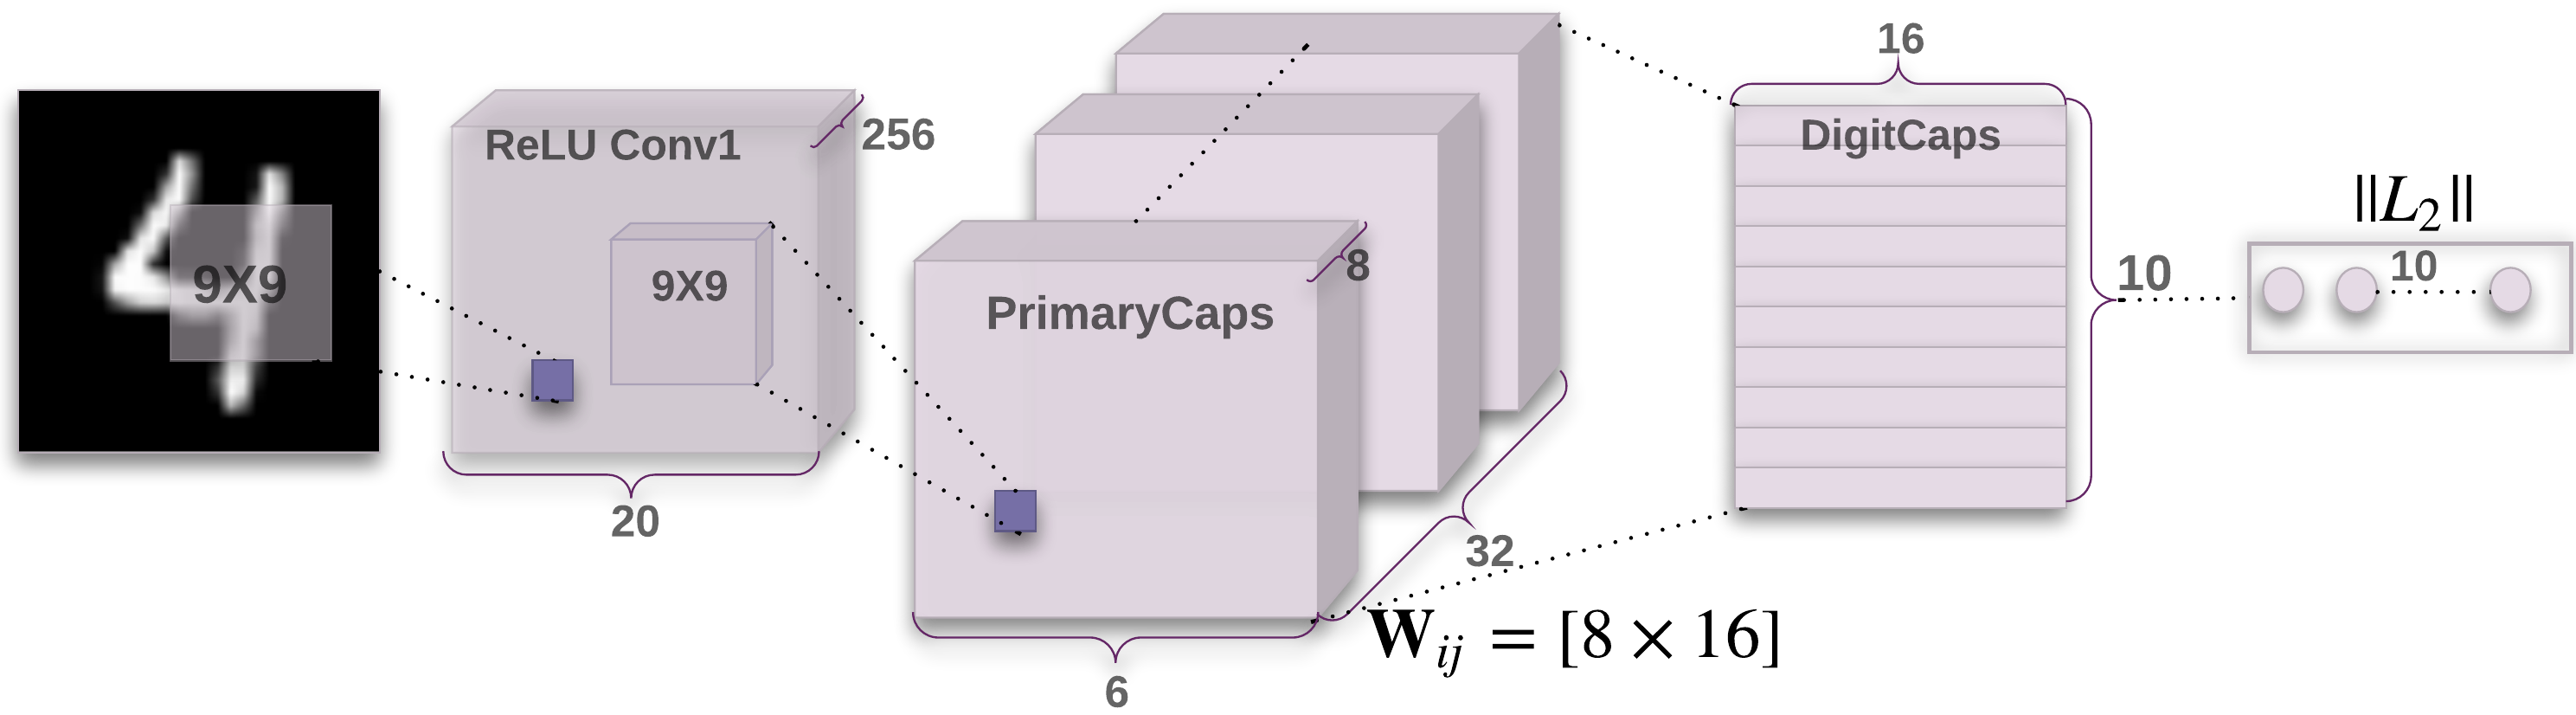
\includegraphics[width=\textwidth]{../img/capsulearch.png}
      \end{center}
    \end{frame}
  }

  \subsection{What is a capsule?}
  {
    \setbeamertemplate{frame footer}{\colorcite[\cite{Sabour2017dynamic}]}
  }

%%%%%%%%%%%%%%%%%%%%%%%%%%%%%%%%%%%%%%%%%%%%%%%%%%%%%%%%%%%%%%%%%%%%%%%%%%%%%%%%

  \section{Routing by an Agreement}

  \subsection{Algorithm}
  {
    \setbeamertemplate{frame footer}{\colorcite\url{https://www.oreilly.com/ideas/introducing-capsule-networks}}

    \begin{frame}{Routing by an Agreement: High-Dimensional Coincidence}
      \pause
      \begin{center}
        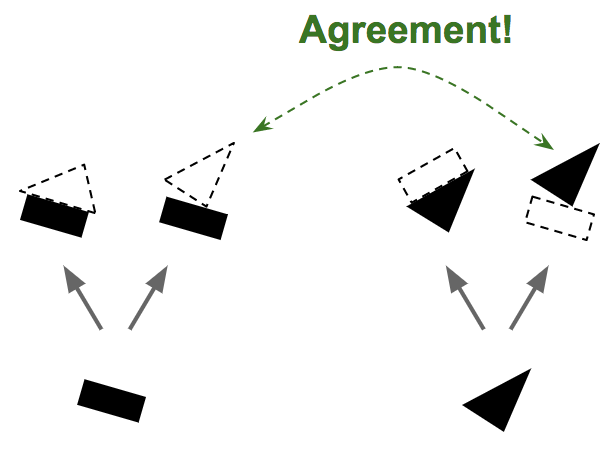
\includegraphics[height=.5\textheight]{../img/routing-agreement.png}
        \pause

        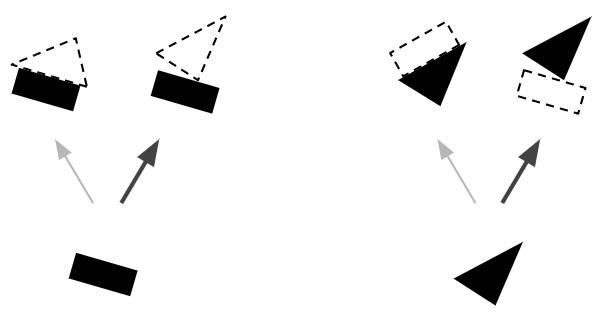
\includegraphics[height=.35\textheight]{../img/routing-weights.png}
      \end{center}
    \end{frame}

    \begin{frame}{Routing by an Agreement: Illustrative Overview}
      \begin{center}
        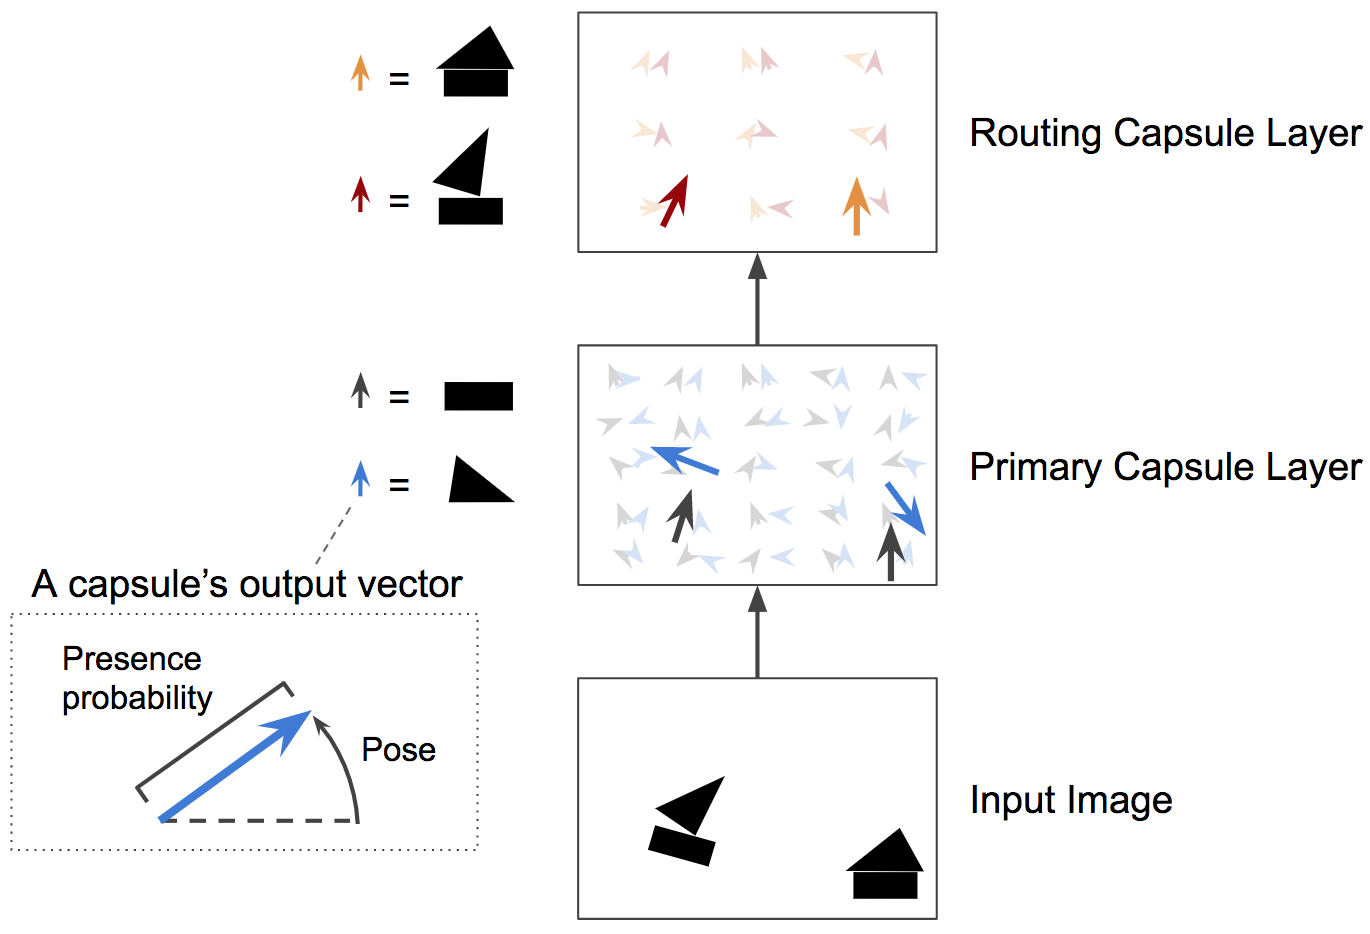
\includegraphics[height=.85\textheight]{../img/routing-by-layers.png}
      \end{center}
    \end{frame}

    \begin{frame}{Routing by an Agreement: Recognizing Ambiguity in Images}
      \begin{center}
        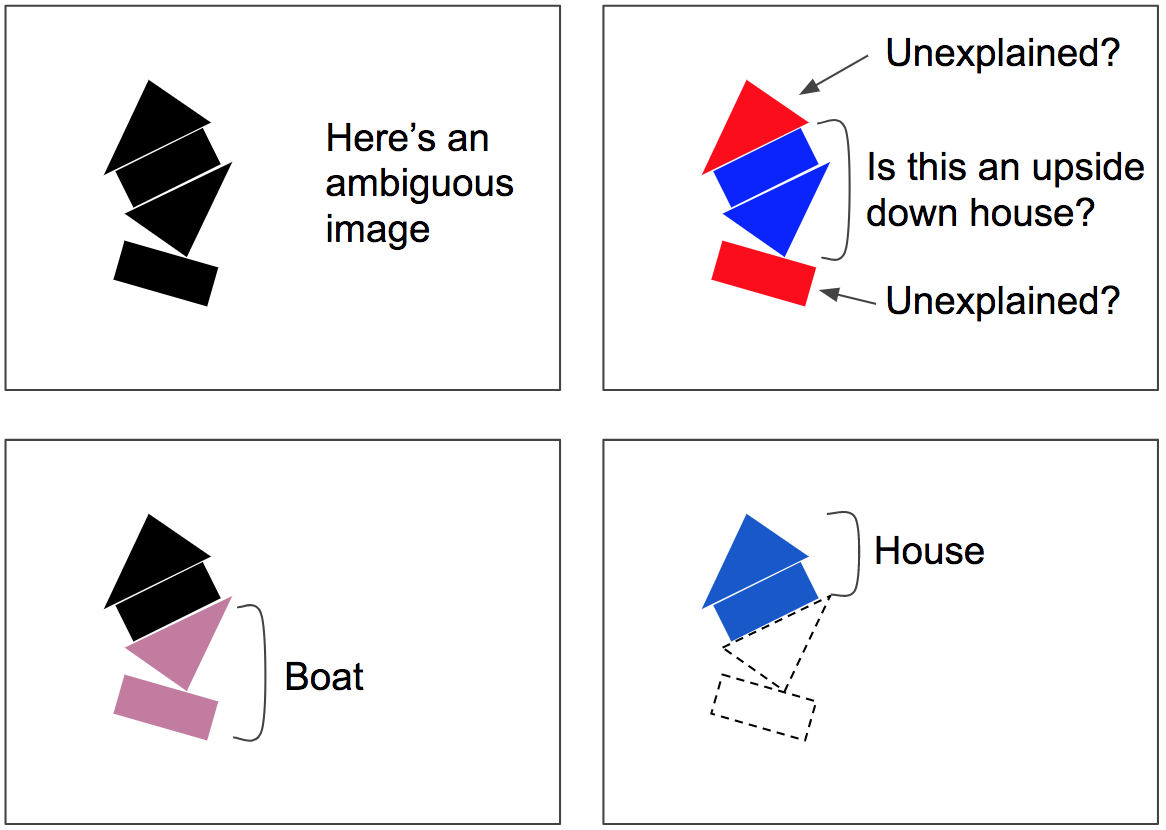
\includegraphics[height=.85\textheight]{../img/ambiguous-shapes.png}
      \end{center}
    \end{frame}
  }

  {
    \setbeamertemplate{frame footer}{\colorcite[\cite{Sabour2017dynamic}]}

    \begin{frame}{Capsule Schema with Routing}
      \begin{center}
        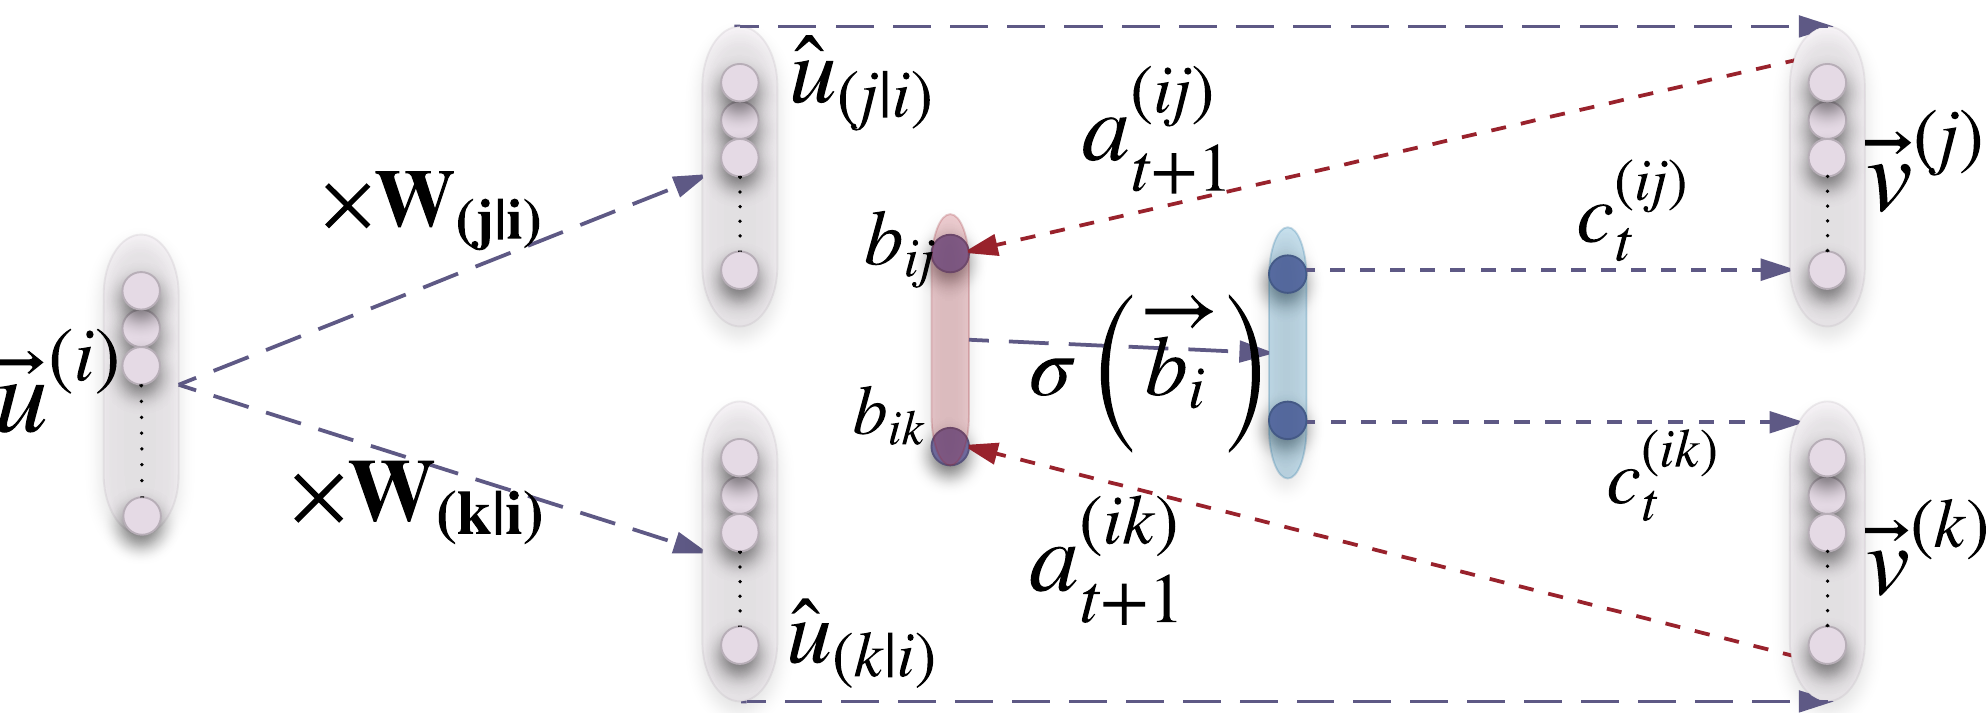
\includegraphics[width=\textwidth]{../img/capsRouting.png}
      \end{center}
    \end{frame}

    \begin{frame}{Routing Softmax}
      \begin{center}
        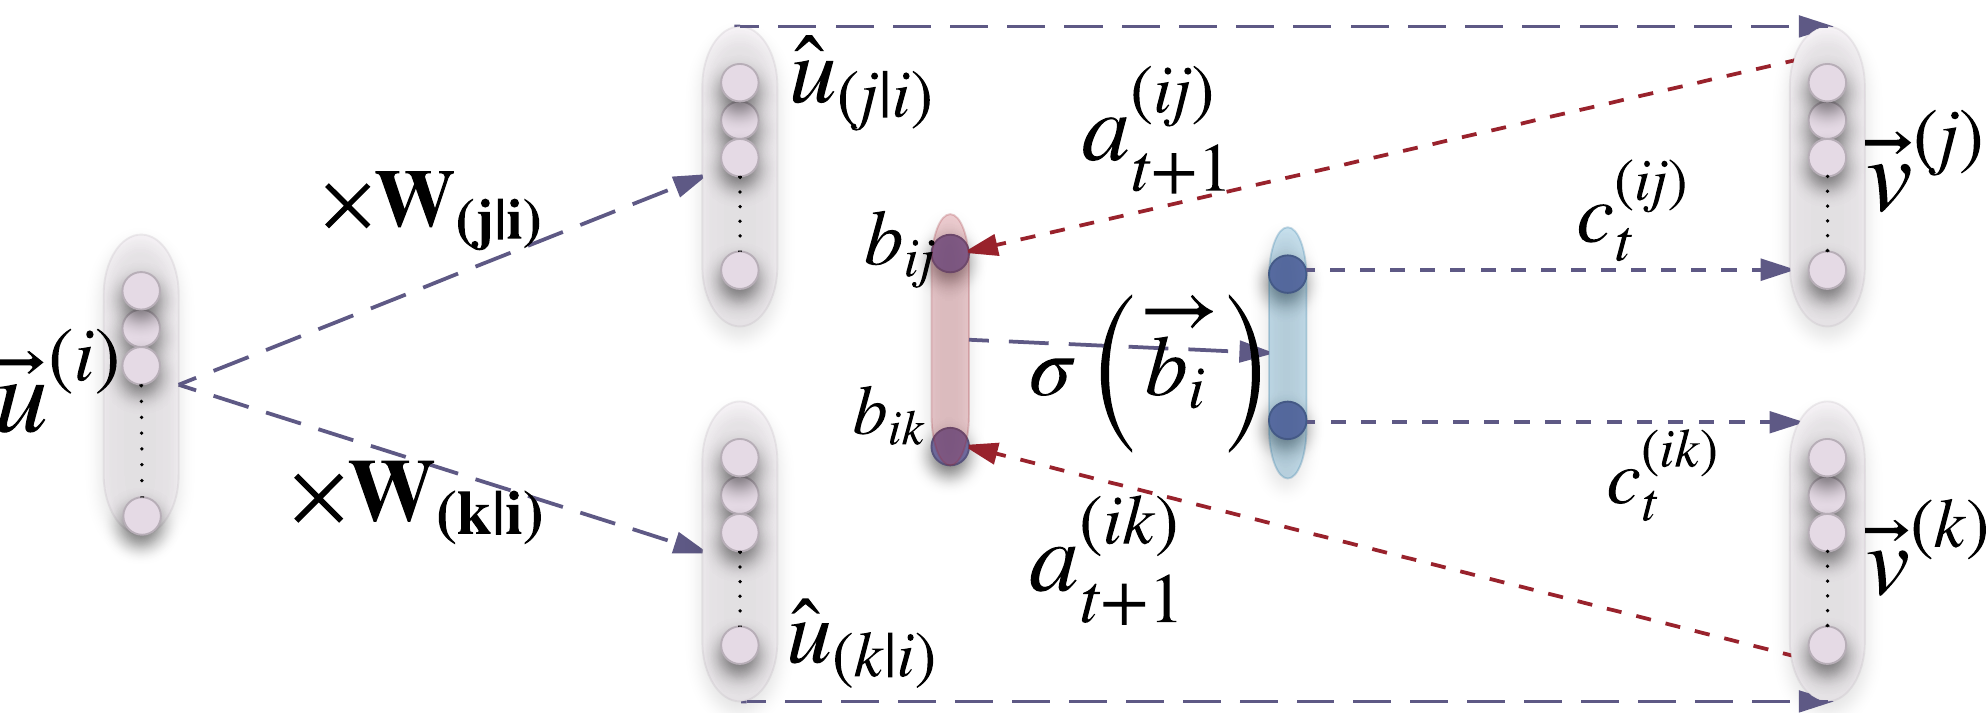
\includegraphics[width=.6\textwidth]{../img/capsRouting.png}
      \end{center}
      \pause

      \begin{equation}
        c_{ij} = \frac{\exp(b_{ij})}{\sum_k \exp(b_{ik})}
        \label{eq:softmax}
      \end{equation}
    \end{frame}

    \begin{frame}{Prediction Vectors}
      \begin{center}
        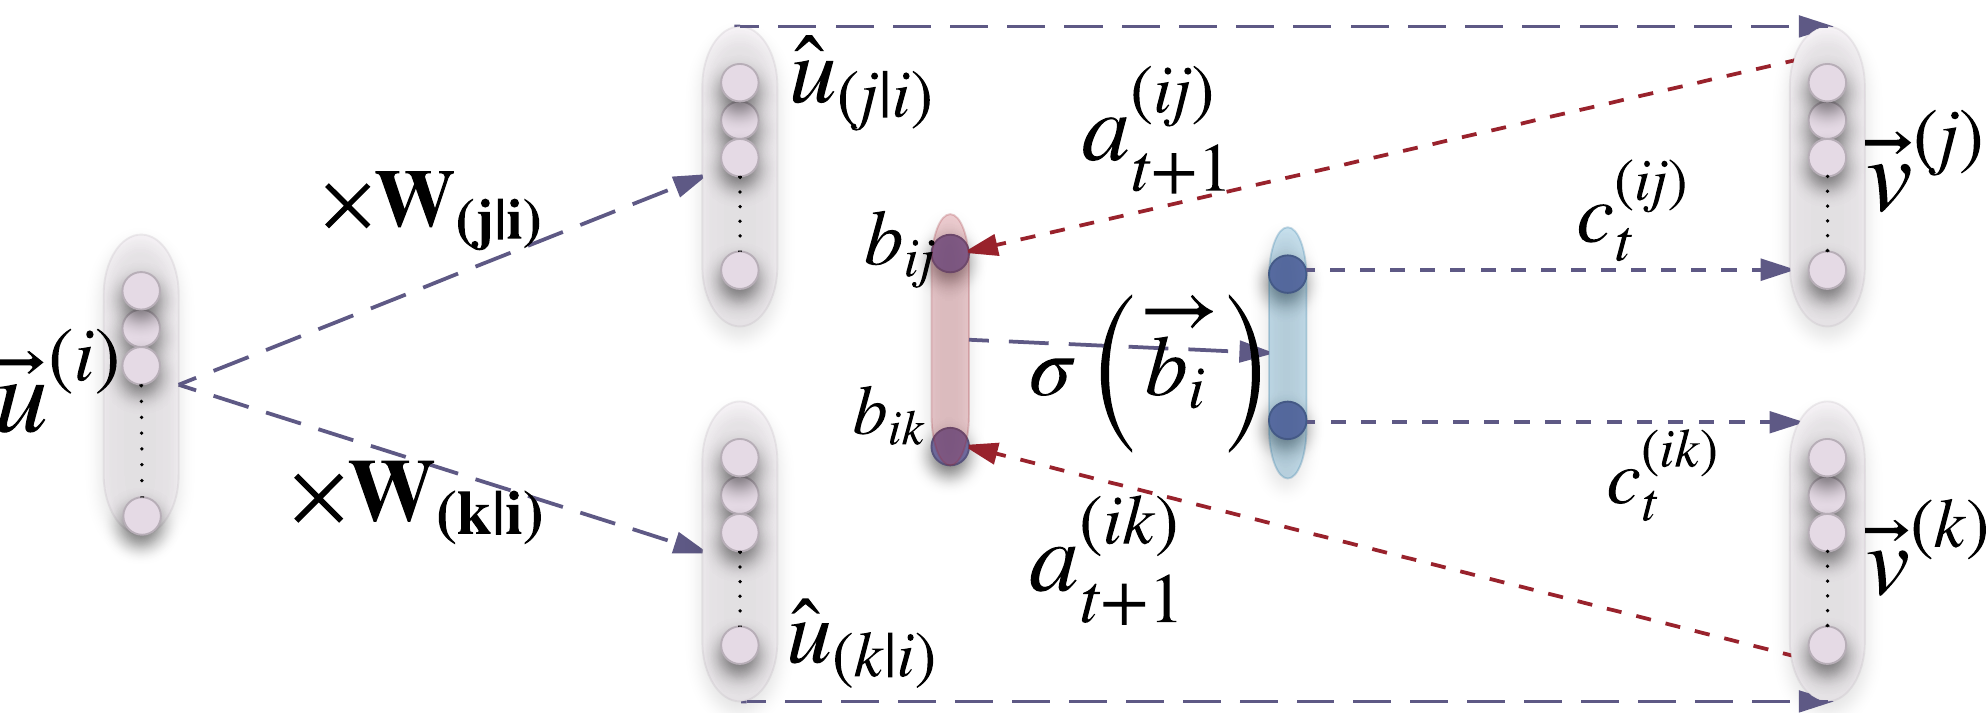
\includegraphics[width=.6\textwidth]{../img/capsRouting.png}
      \end{center}
      \pause

      \begin{equation}
        {\bf \hat{u}}_{j|i} = {\bf W}_{ij}{\bf u}_i 
        \label{eq:predict-vecs}
      \end{equation}
    \end{frame}

    \begin{frame}{Total Input}
      \begin{center}
        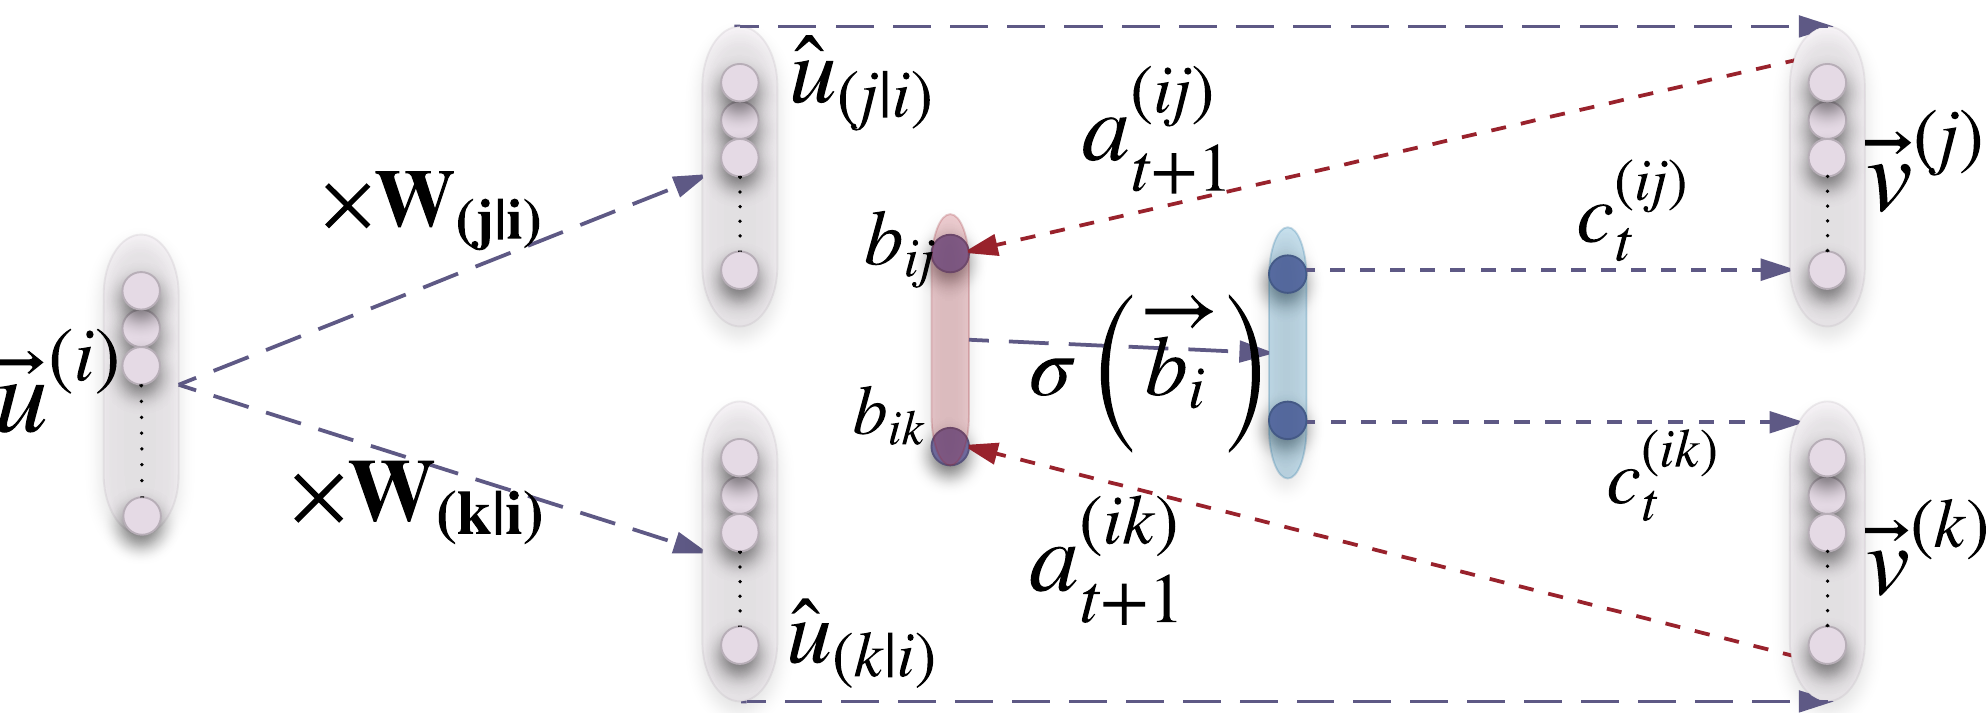
\includegraphics[width=.6\textwidth]{../img/capsRouting.png}
      \end{center}
      \pause

      \begin{equation}
        {\bf s}_j = \sum_i c_{ij} {\bf \hat{u}}_{j|i}
        \label{eq:total-input}
      \end{equation}
    \end{frame}

    \begin{frame}{Squashing}
      \begin{center}
        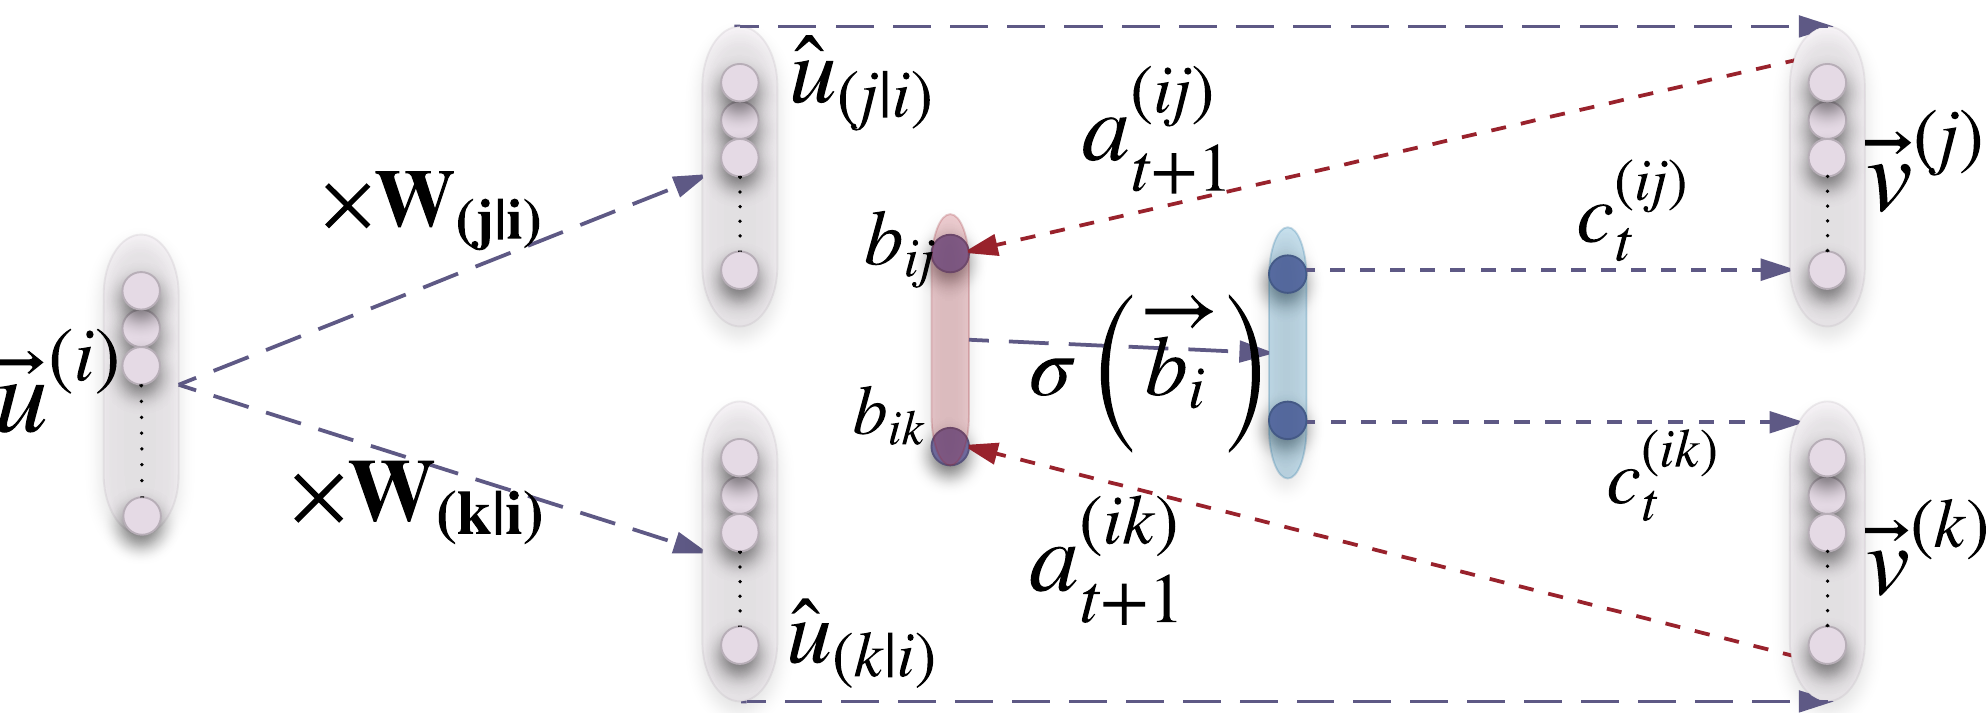
\includegraphics[width=.6\textwidth]{../img/capsRouting.png}
      \end{center}
      \pause

      \begin{equation}
        {\bf v}_j = \frac{||{\bf s}_j||^2}{1+||{\bf s}_j||^2} \frac{{\bf s}_j}{||{\bf s}_j||}
        \label{eq:squash}
      \end{equation}
      \pause
      \begin{center}
        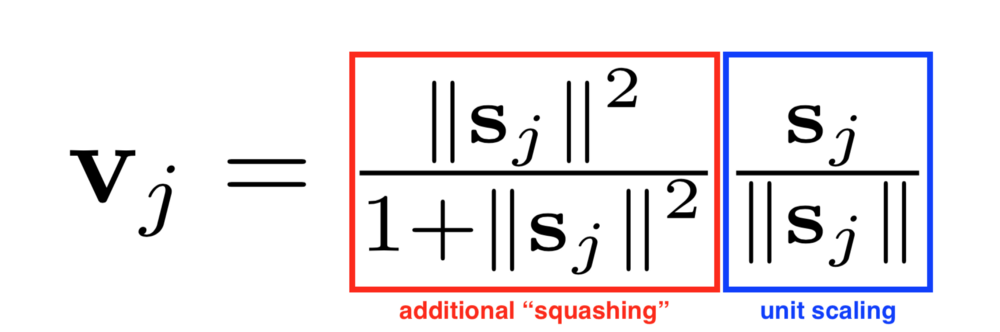
\includegraphics[width=.7\textwidth]{../img/squashing.png}
      \end{center}
    \end{frame}

    \begin{frame}{Routing Algorithm}
      \begin{center}
        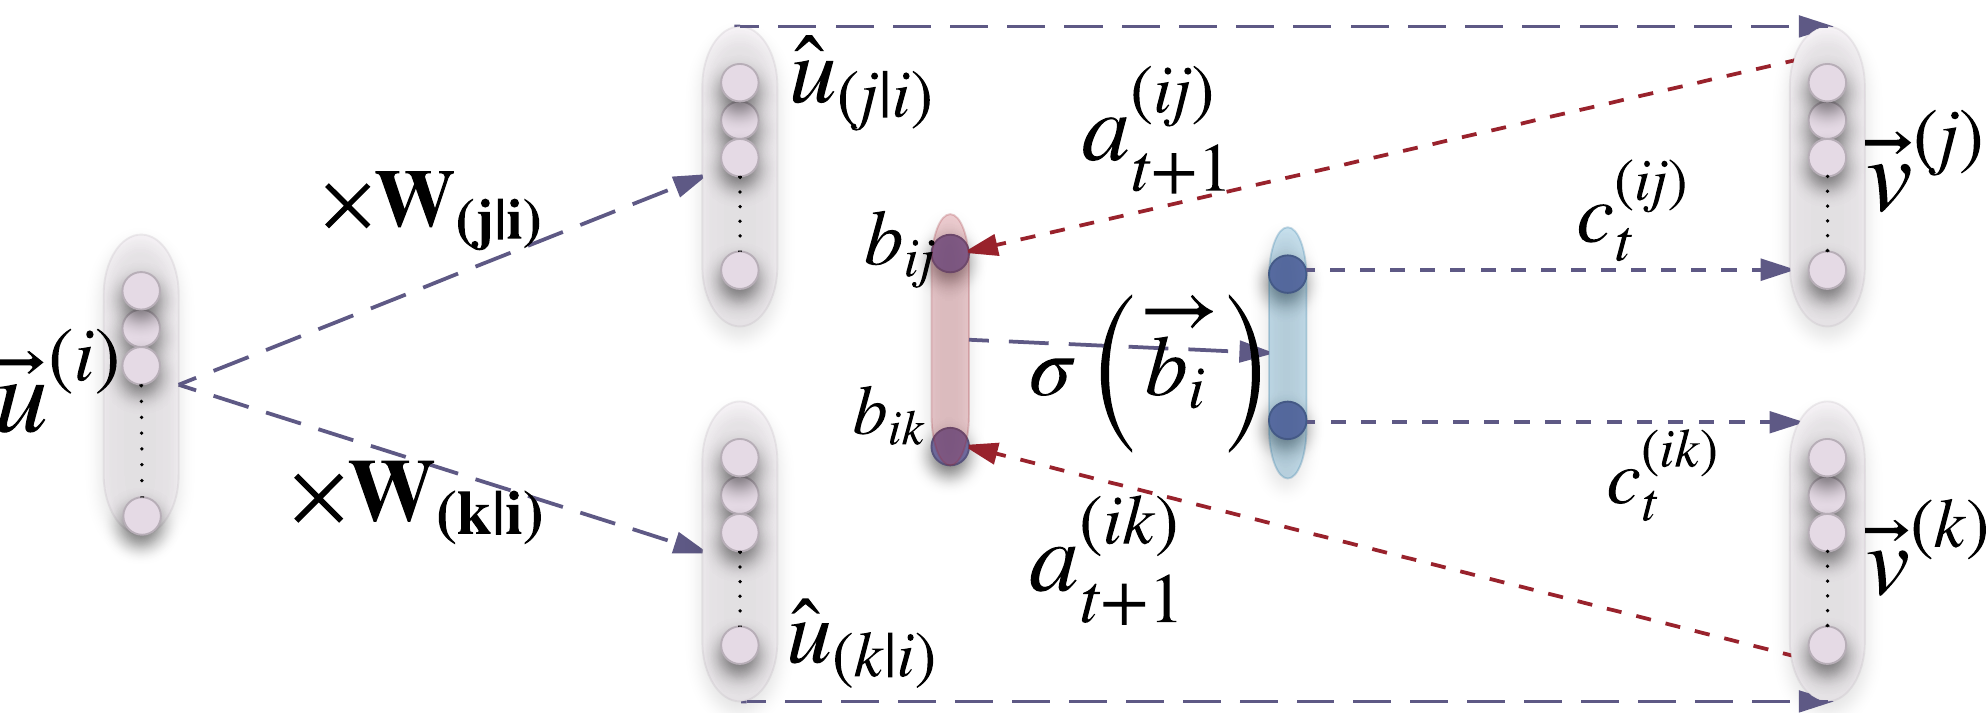
\includegraphics[width=.6\textwidth]{../img/capsRouting.png}
      \end{center}
      \pause

      \begin{algorithm}[H]
        \caption{Dynamic Routing between Capsules}
        \scriptsize
        \begin{algorithmic}[1]
          \Procedure{Routing}{$\bm{\hat{u}}_{j|i}$, $r$, $l$}
          \pause
          \State for all capsule $i$ in layer $l$ and capsule $j$ in layer $(l+1)$: $b_{ij} \gets 0$.
          \pause
          \For{$r$ iterations}
          \pause
          \State for all capsule $i$ in layer $l$: ${\bf c}_i \gets \texttt{softmax}({\bf b}_i)$ \Comment{\texttt{softmax} computes Eq.~\ref{eq:softmax}}
          \pause
          \State for all capsule $j$ in layer $(l+1)$: ${\bf s}_j \gets \sum_i{c_{ij}{\bf \hat u}_{j|i}}$ \Comment{total input from Eq.~\ref{eq:total-input}}
          \pause
          \State for all capsule $j$ in layer $(l+1)$: ${\bf v}_j \gets \texttt{squash}({\bf s}_j)$ \Comment{\texttt{squash} computes Eq.~\ref{eq:squash}}
          \pause
          \State for all capsule $i$ in layer $l$ and capsule $j$ in layer $(l+1)$: $b_{ij} \gets b_{ij} + {\bf \hat{u}}_{j|i} . {\bf v}_j$
          \pause
          \EndFor
          \Return ${\bf v}_j$
          \EndProcedure
        \end{algorithmic}
      \end{algorithm}
    \end{frame}
  }
  
  {
    \setbeamertemplate{frame footer}{\colorcite\url{https://youtu.be/rTawFwUvnLE}}

    \usebackgroundtemplate{
      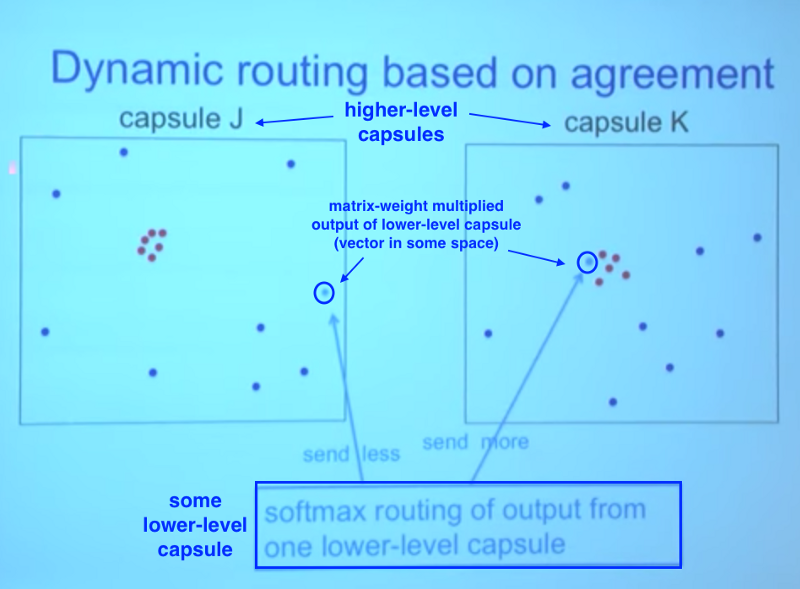
\includegraphics[height=\paperheight]{../img/hi-dim-coincidence-hinton.png}
    }
    \begin{frame}[standout]
    \end{frame}
  }

  {
    \setbeamertemplate{frame footer}{\colorcite\url{https://github.com/naturomics/CapsNet-Tensorflow}}

    \usebackgroundtemplate{
      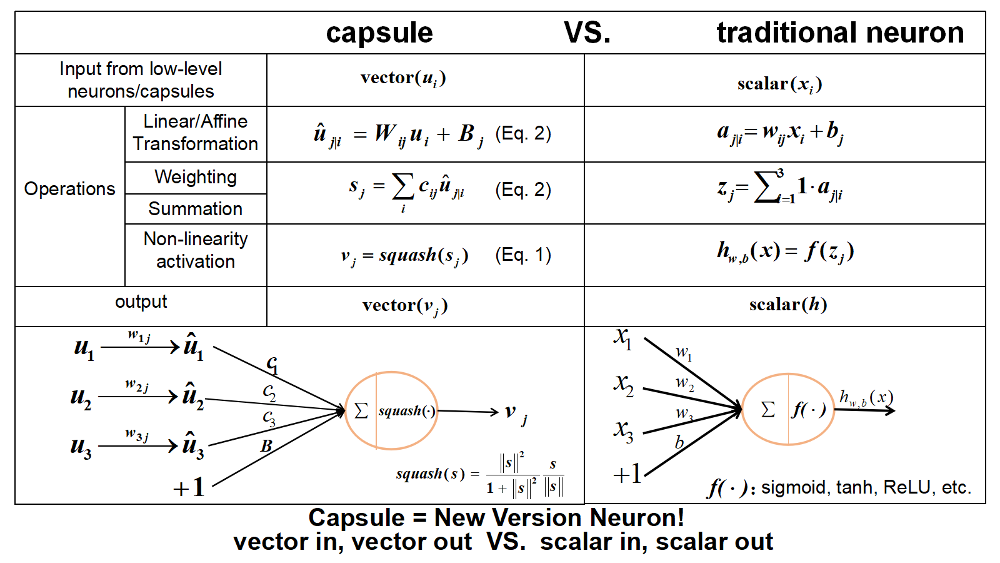
\includegraphics[width=\paperwidth]{../img/capsuleVSneuron.png}
    }
    \begin{frame}[standout]
    \end{frame}
  }

  \subsection{Routing Iterations}
  {
    \setbeamertemplate{frame footer}{\colorcite[\cite{Sabour2017dynamic}]}

    \begin{frame}{Average Change of Each Routing Logit $b_{ij}$ \\
        \tiny (by each routing iteration during training)}
      \pause
      \begin{center}
        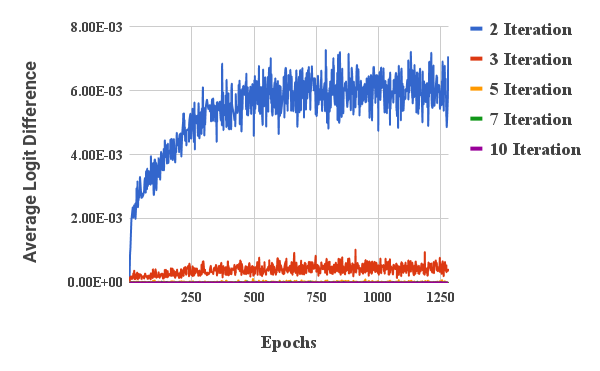
\includegraphics[width=\textwidth]{../img/conv}
      \end{center}
    \end{frame}

    \begin{frame}{Log Scale of Final Differences}
      \begin{center}
        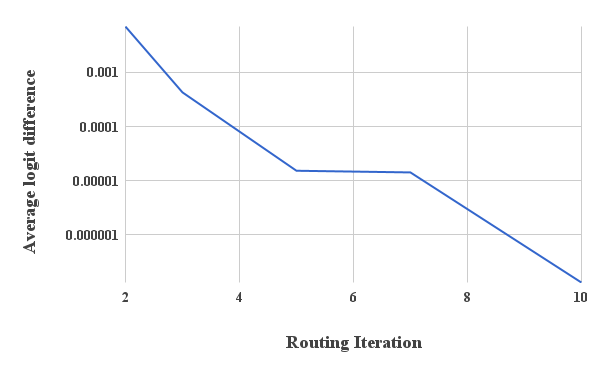
\includegraphics[width=\textwidth]{../img/c_e1}
      \end{center}
    \end{frame}


    \begin{frame}{Training Loss of CapsNet on CIFAR10 \\
        \tiny (batch size of $128$)}
      The CapsNet with \alert{$3$ routing iterations} optimizes the loss faster and converges to a~lower loss at the end.
      \pause

      \begin{center}
        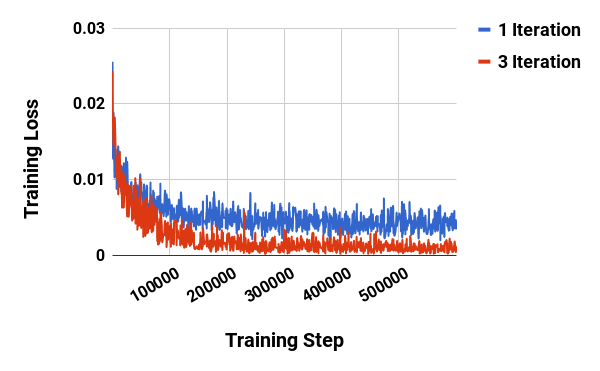
\includegraphics[width=.9\textwidth]{../img/cifar}
      \end{center}
      \pause
    \end{frame}
  }

%%%%%%%%%%%%%%%%%%%%%%%%%%%%%%%%%%%%%%%%%%%%%%%%%%%%%%%%%%%%%%%%%%%%%%%%%%%%%%%%

  \section{Capsule Network}

  \subsection{Loss}
  {
    \setbeamertemplate{frame footer}{\colorcite[\cite{Sabour2017dynamic}]}

    \begin{frame}{Margin Loss \\
        \tiny for Digit Existence}
      For each digit capsule $k$, its loss $L_k$ is:
      \pause
      \begin{equation*}
        L_k =
        \begin{dcases*} 
          \max(0, m^{+} - ||{\bf v}_k||)^2            & iff a digit of class $k$ is present \\
          \lambda \max(0, ||{\bf v}_k|| - m^{-})^2    & otherwise
        \end{dcases*}
      \end{equation*}
      where
      \pause
      \begin{itemize}[<+- | alert@+>]
        \item $m^{+} = 0.9$
        \item $m^{-} = 0.1$
        \item $\lambda = 0.5$ is down-weighting of the loss for absent digit classes.
          {\tiny It stops the initial learning from shrinking the lengths of the activity vectors.}
        \item The total loss is the sum of the losses of all digit capsules.
      \end{itemize}
    \end{frame}
  }

  \subsection{Architecture}
  {
    \setbeamertemplate{frame footer}{\colorcite[\cite{Sabour2017dynamic}]}

    \begin{frame}{Simple CapsNet with 3 Layers}
      \begin{center}
        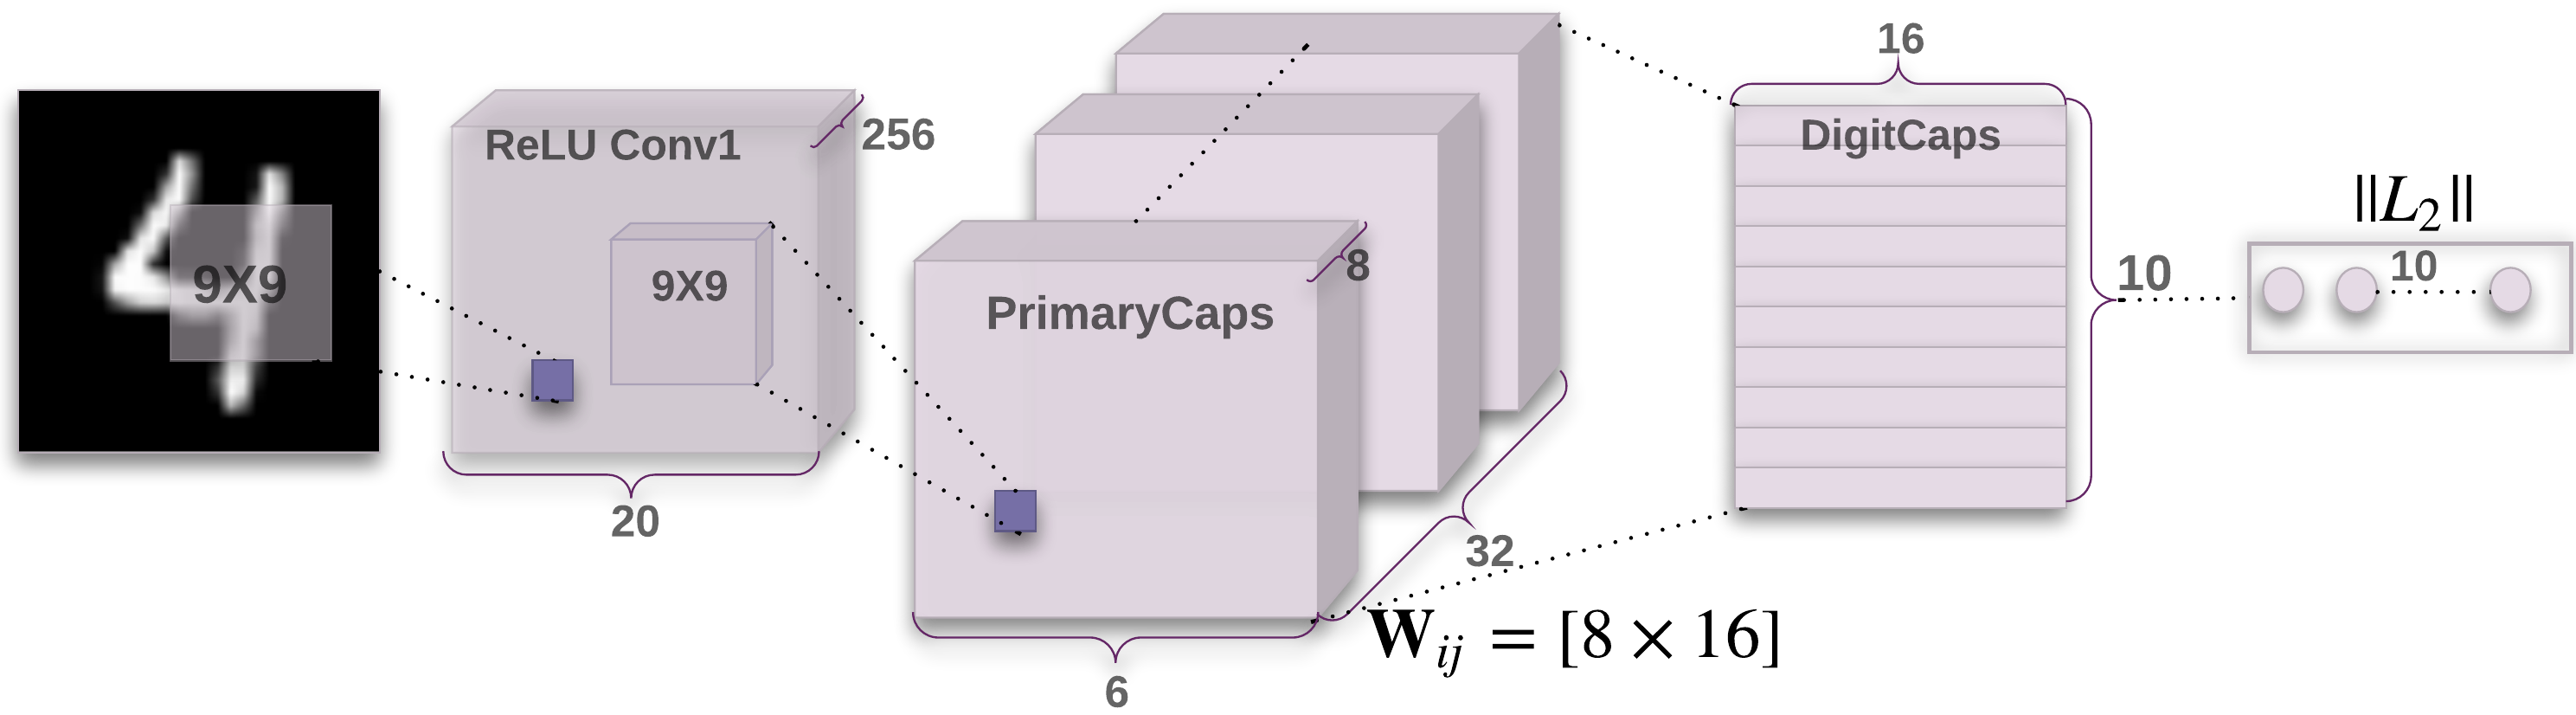
\includegraphics[width=\textwidth]{../img/capsulearch.png}
      \end{center}
    \end{frame}

    \begin{frame}{Decoder to Reconstruct a Digit from DigitCaps}
      \begin{center}
        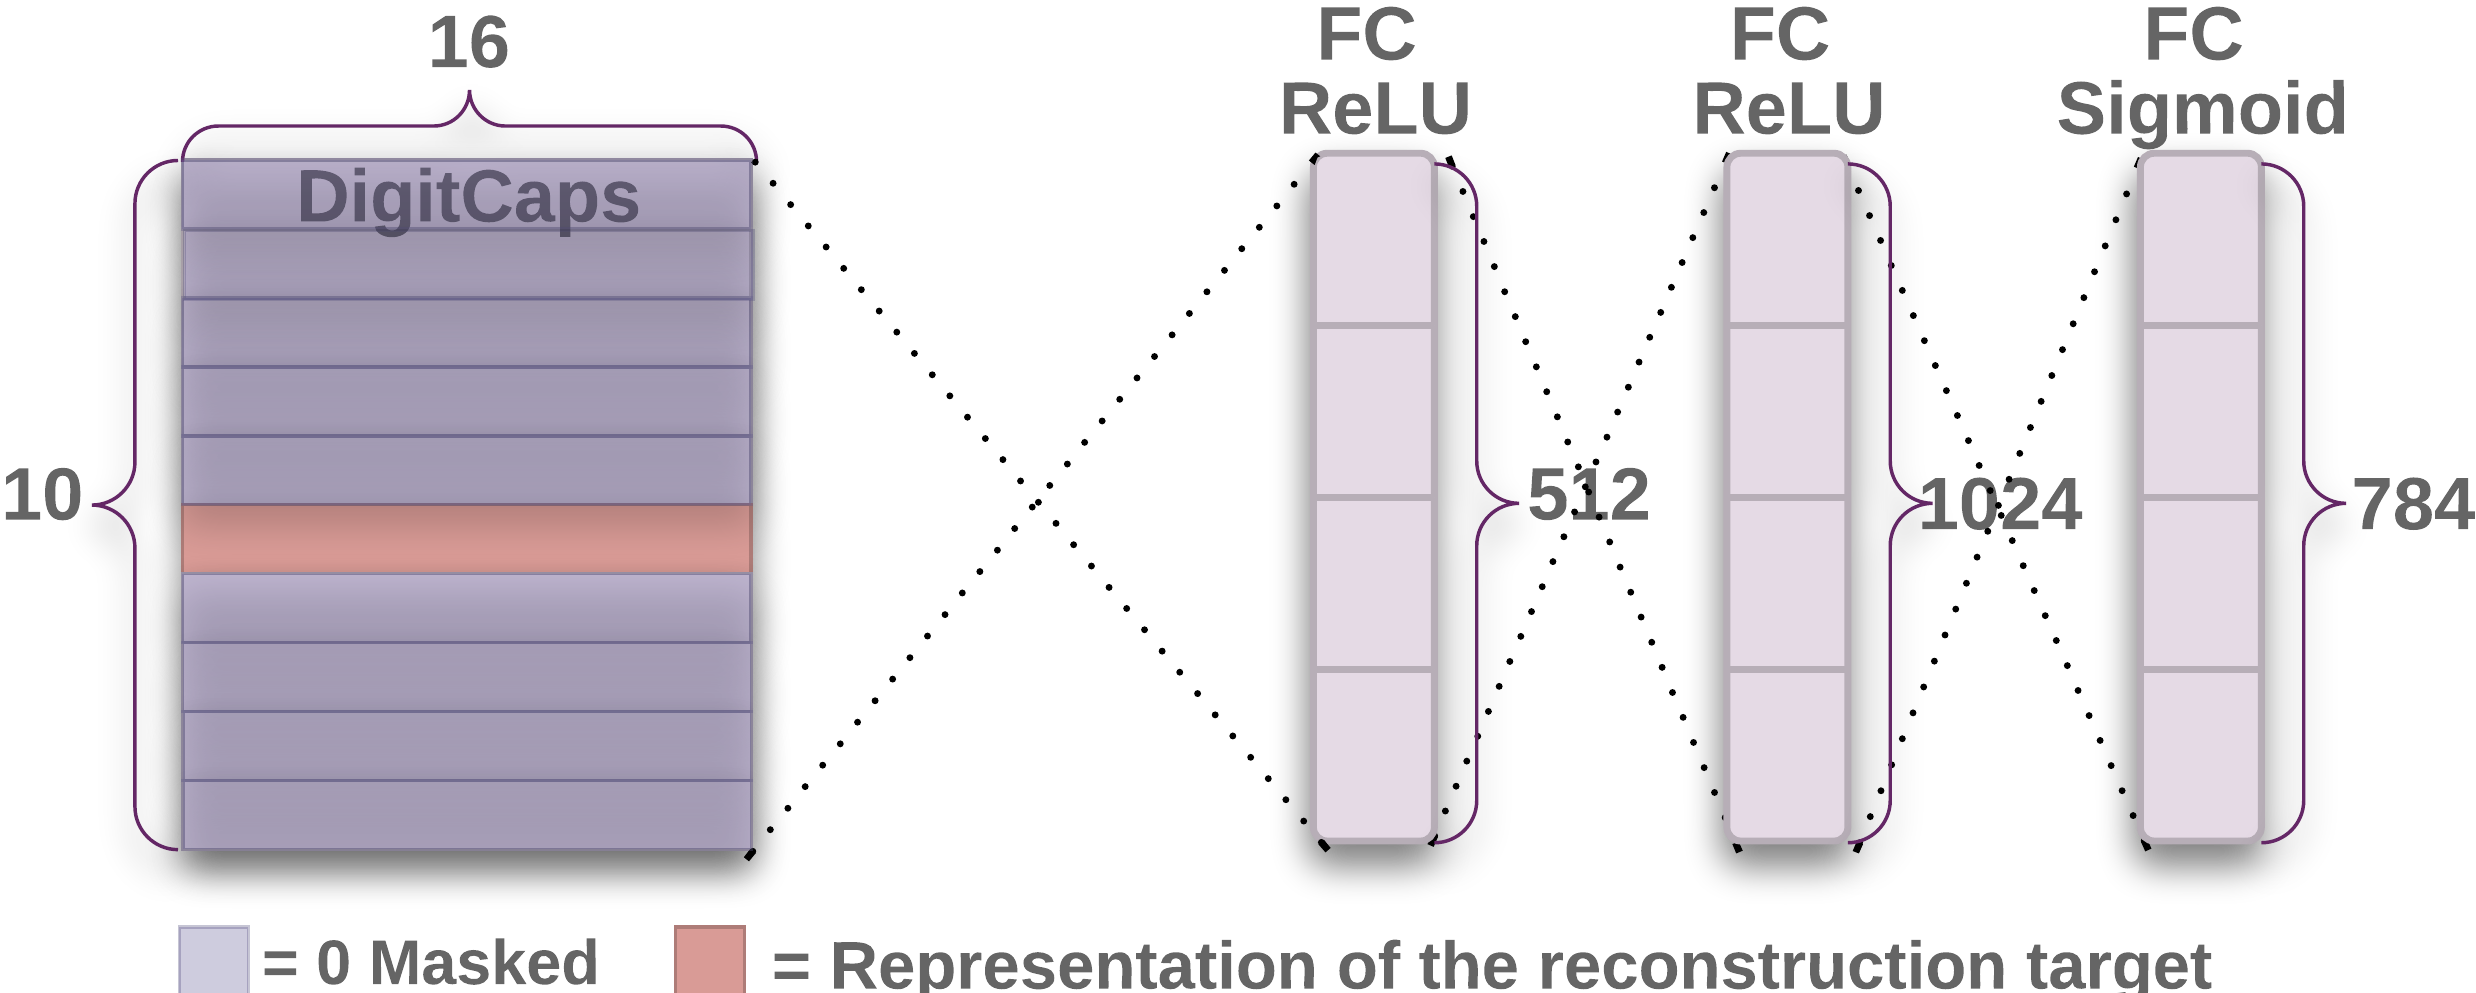
\includegraphics[width=\textwidth]{../img/reconsArch.png}
      \end{center}
    \end{frame}
  }

%%%%%%%%%%%%%%%%%%%%%%%%%%%%%%%%%%%%%%%%%%%%%%%%%%%%%%%%%%%%%%%%%%%%%%%%%%%%%%%%

  \section{Experiments}

  \subsection{MNIST}
  {
    \setbeamertemplate{frame footer}{\colorcite[\cite{Sabour2017dynamic}]}

    \begin{frame}{MNIST Reconstructions (CapsNet, 3 routing iterations)}
      \begin{tabular}
        { r | c c | c c}
        Label:          & 8 & 5 & 5 & 5 \\
        Prediction:     & 8 & 5 & 3 & 3 \\
        Reconstruction: & 8 & 5 & 5 & 3 \\
        \pbox{.2\textwidth}{\hspace{1em}Input: \\ \\ \\ Output:} &
        \pbox{.2\textwidth}{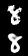
\includegraphics[width=.15\textwidth]{../img/recons/8_226}} &
        \pbox{.2\textwidth}{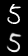
\includegraphics[width=.15\textwidth]{../img/recons/5_153}} &
        \pbox{.2\textwidth}{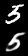
\includegraphics[width=.15\textwidth]{../img/recons/5_2035}} &
        \pbox{.2\textwidth}{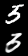
\includegraphics[width=.15\textwidth]{../img/recons/5_2035p}}
      \end{tabular}
    \end{frame}

    \begin{frame}{Dimension perturbations}
      one of the $16$ dimensions, by intervals of $0.05$ in the range $[-0.25, 0.25]$:
      \pause

      \begin{tabular}{r | r}
        Interpretation & Reconstructions after perturbing \\
        \hline
        ``scale and thickness'' & 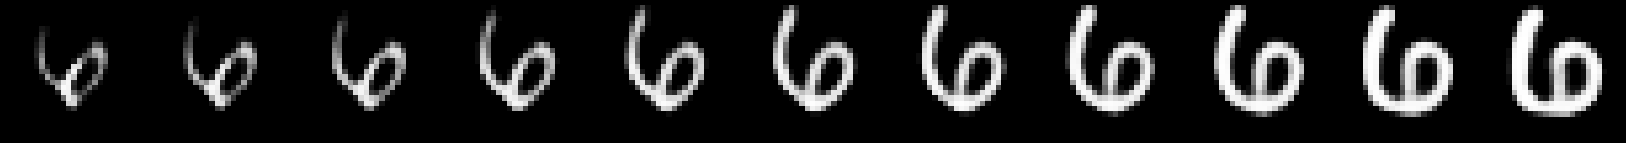
\includegraphics[width=7cm]{../img/recons/dim6} \\
        ``localized part'' & 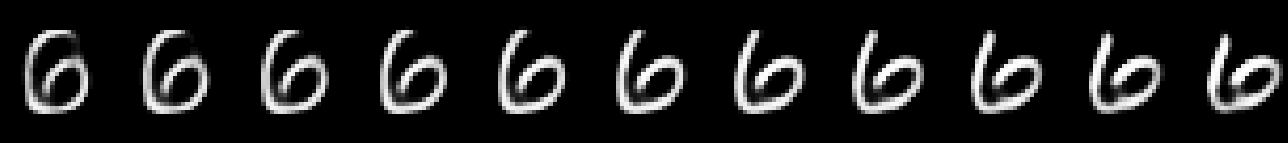
\includegraphics[width=7cm]{../img/recons/dim7} \\
        \pause
        ``stroke thickness'' & 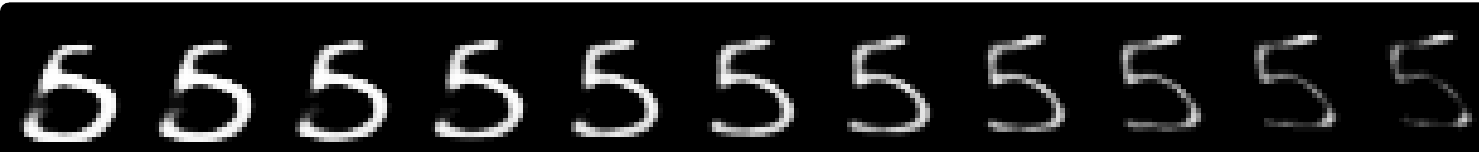
\includegraphics[width=7cm]{../img/recons/dim8} \\
        ``localized skew'' & 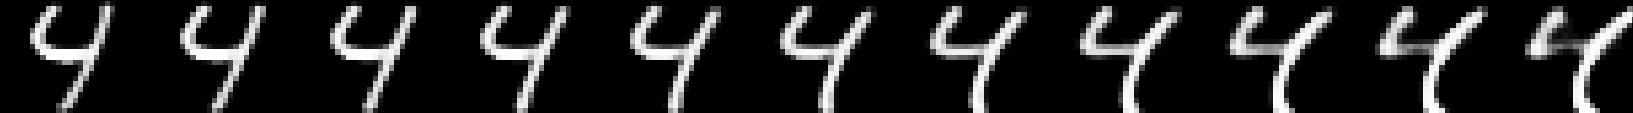
\includegraphics[width=7cm]{../img/recons/dim12} \\
        \pause
        ``width and translation'' & 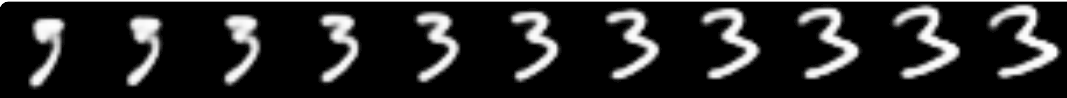
\includegraphics[width=7cm]{../img/recons/dim10} \\
        ``localized part'' & 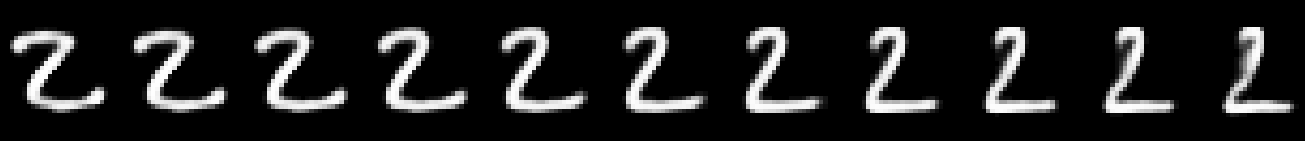
\includegraphics[width=7cm]{../img/recons/dim11}
      \end{tabular}
    \end{frame}
  }

  \subsection{MultiMNIST}
  {
    \setbeamertemplate{frame footer}{\colorcite[\cite{Sabour2017dynamic}]}

    \begin{frame}{MultiMNIST Reconstructions (CapsNet, 3 routing iterations)}
      \begin{center}
        \begin{tabular}{c c c c}
          R:$(2,7)$ & R:$(6,0)$ & R:$(6,8)$ & R:$(7,1)$ \\
          L:$(2,7)$ & L:$(6,0)$ & L:$(6,8)$ & L:$(7,1)$ \\ \hline
          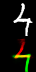
\includegraphics[height=.3\textheight]{../img/recons/27} &
          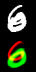
\includegraphics[height=.3\textheight]{../img/recons/60} &
          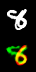
\includegraphics[height=.3\textheight]{../img/recons/68} &
          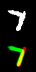
\includegraphics[height=.3\textheight]{../img/recons/71} \\
          \pause
          *R:$(5,7)$ & *R:$(2,3)$ & R:$(2,8)$ & R:P:$(2,7)$ \\
           L:$(5,0)$ &  L:$(4,3)$ & L:$(2,8)$ & L:$(2,8)$ \\ \hline
          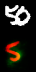
\includegraphics[height=.3\textheight]{../img/recons/0_5_5_0_332} &
          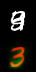
\includegraphics[height=.3\textheight]{../img/recons/4_3_3_4_397} &
          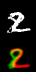
\includegraphics[height=.3\textheight]{../img/recons/2_8_2_7_152} &
          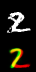
\includegraphics[height=.3\textheight]{../img/recons/2_8_2_7_153p}
        \end{tabular}
      \end{center}
    \end{frame}

    \begin{frame}{MultiMNIST Reconstructions (CapsNet, 3 routing iterations)}
      \begin{center}
        \begin{tabular}{c c c c}
          R:$(8,7)$ & R:$(9,4)$ & R:$(9,5)$ & R:$(8,4)$ \\
          L:$(8,7)$ & L:$(9,4)$ & L:$(9,5)$ & L:$(8,4)$ \\ \hline
          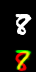
\includegraphics[height=.3\textheight]{../img/recons/87} &
          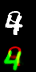
\includegraphics[height=.3\textheight]{../img/recons/94} &
          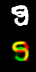
\includegraphics[height=.3\textheight]{../img/recons/95} &
          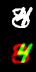
\includegraphics[height=.3\textheight]{../img/recons/84} \\
          \pause
          *R:$(0,8)$ & *R:$(1,6)$ & R:$(4,9)$ &  R:P:$(4, 0)$ \\
           L:$(1,8)$ &  L:$(7,6)$ & L:$(4, 9)$ & L:$(4, 9)$ \\ \hline
          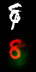
\includegraphics[height=.3\textheight]{../img/recons/1_8_8_1_264} &
          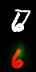
\includegraphics[height=.3\textheight]{../img/recons/7_6_6_7_4} &
          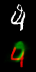
\includegraphics[height=.3\textheight]{../img/recons/4_9_4_0_453} &
          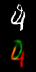
\includegraphics[height=.3\textheight]{../img/recons/4_9_4_0_454p}
        \end{tabular}
      \end{center}
    \end{frame}

  \subsection{CIFAR10}

  \subsection{smallNORB}

  \subsection{SVHN}

%%%%%%%%%%%%%%%%%%%%%%%%%%%%%%%%%%%%%%%%%%%%%%%%%%%%%%%%%%%%%%%%%%%%%%%%%%%%%%%%

  \section{Conclusion}

  \subsection{Explanation of Capsules' Efficiency}

  \begin{frame}[standout]
    \begin{center}
      Thank you!

      Questions?
    \end{center}
  \end{frame}

%%%%%%%%%%%%%%%%%%%%%%%%%%%%%%%%%%%%%%%%%%%%%%%%%%%%%%%%%%%%%%%%%%%%%%%%%%%%%%%%

  \appendix
  \begin{frame}[standout]
    Backup Slides
  \end{frame}

  % TODO display (I), (II) instead of i, ii
  \begin{frame}[allowframebreaks]{Further Reading}
    \tiny
    Artificial Intelligence:
    \begin{itemize}
      \item \textbf{Artificial Intelligence course at MIT} \url{http://ocw.mit.edu/courses/electrical-engineering-and-computer-science/6-034-artificial-intelligence-fall-2010/index.htm}
      \item \textbf{Introduction to Artificial Intelligence at Udacity} \url{https://www.udacity.com/course/intro-to-artificial-intelligence--cs271}
      \item \textbf{General Game Playing course} \url{https://www.coursera.org/course/ggp}
      \item \textbf{Singularity} \url{http://waitbutwhy.com/2015/01/artificial-intelligence-revolution-1.html} + Part 2
      \item \textbf{The Singularity Is Near} (\cite{Kurzweil2005singularity})
    \end{itemize}

    Machine Learning:
    \begin{itemize}
      \item \textbf{Machine Learning course} \url{https://youtu.be/hPKJBXkyTK://www.coursera.org/learn/machine-learning/}
      \item \textbf{Reinforcement Learning} \url{http://reinforcementlearning.ai-depot.com/}
      \item \textbf{Deep Learning} (\cite{Lecun2015deep})
      \item \textbf{Deep Learning course} \url{https://www.udacity.com/course/deep-learning--ud730}
      \item \textbf{Two Minute Papers} \url{https://www.youtube.com/user/keeroyz}
      \item \textbf{Applications of Deep Learning} \url{https://youtu.be/hPKJBXkyTKM}
    \end{itemize}

    Neuroscience:
    \begin{itemize}
      \item \url{http://www.brainfacts.org/}
    \end{itemize}
  \end{frame}

  \begin{frame}[allowframebreaks]{References}
    \tiny
    \printbibliography[heading=none]
  \end{frame}

\end{document}
